\documentclass{article}

% if you need to pass options to natbib, use, e.g.:
% \PassOptionsToPackage{numbers, compress}{natbib}
% before loading nips_2017
%
% to avoid loading the natbib package, add option nonatbib:
% \usepackage[nonatbib]{nips_2017}

\usepackage[final]{nips_2017}

% to compile a camera-ready version, add the [final] option, e.g.:
% \usepackage[final]{nips_2017}

\usepackage[utf8]{inputenc} % allow utf-8 input
\usepackage[T1]{fontenc}    % use 8-bit T1 fonts
\usepackage{hyperref}       % hyperlinks
\usepackage{url}            % simple URL typesetting
\usepackage{booktabs}       % professional-quality tables
\usepackage{amsfonts}       % blackboard math symbols
\usepackage{nicefrac}       % compact symbols for 1/2, etc.
\usepackage{microtype}      % microtypography
\usepackage{cite}
\usepackage{amsmath}
\usepackage{graphicx} 

\usepackage{algorithm}  
\usepackage{algpseudocode}  
\usepackage{amsmath}  
\renewcommand{\algorithmicrequire}{\textbf{Input:}}  % Use Input in the format of Algorithm  
\renewcommand{\algorithmicensure}{\textbf{Output:}} % Use Output in the format of Algorithm  

\hypersetup{colorlinks,linkcolor={blue},citecolor={blue},urlcolor={blue}}  

\title{CS150A Database \\Course Project}

% The \author macro works with any number of authors. There are two
% commands used to separate the names and addresses of multiple
% authors: \And and \AND.
%
% Using \And between authors leaves it to LaTeX to determine where to
% break the lines. Using \AND forces a line break at that point. So,
% if LaTeX puts 3 of 4 authors names on the first line, and the last
% on the second line, try using \AND instead of \And before the third
% author name.

\author{
  Student 1\\
  ID: 2020533044\\
  \texttt{jiangych2@shanghaitech.edu.cn} \\
  %% examples of more authors
   \And
  Student 2\\
  ID: 2020533171\\
  \texttt{xuzhy2@shanghaitech.edu.cn}
}

\begin{document}
% \nipsfinalcopy is no longer used

\maketitle

\begin{abstract}

Compared with developing a novel machine learning algorihtm, building a machine learning system is less theoretical but more engineering, so it is important to get your hands dirty. To build an entire machine learning system, you have to go through some essential steps. We have listed 5 steps which we hope you to go through. Read the instructions of each section before you fill in. You are free to add more sections. \\
If you use PySpark to implement the algorithms and want to earn some additional points, you should also report your implementation briefly in the last section.
\end{abstract}

\section{Explore the dataset}
\textcolor{cyan}{Instruction: \\
Explore the given dataset, report your findings about the dataset. You should not repeat the information provided in the 'Data Format' section of project.pdf. Instead, you can report the data type of each feature, the distribution of different values of some important features(maybe with visualization), is there any missing value, etc}\\\\
\textbf{Your work below:}\\
As we explore the training and test data, we have the following discovery:\\
(1) There are more than 230,000 logs of data, and the total number of student is 174;\\
(2) On average, the duration for any problem step was about 18 seconds, and the time for a student to achieve the correct answer is stacked between 0 to 15 seconds;\\
(3) The number of unique problem is approximately 1000, and the difficulty of each problem varies, which could be indicated by the median time to solve one certain problem;\\
(4) The columns could be divided into discrete data(e.g. student id, problem hierarchy, etc.) and real-number data(e.g. opportunity). The former needs to be vectorized and encoded in our preprocessing phase;\\
(5) Some missing features in test.csv are useless in our training dataset, these columns need to be dropped for feature engineering.



\section{Data cleaning}
\textcolor{cyan}{Instruction: \\
Some people treat data cleaning as a part of feature engineering, however we separate them here to make your work clearer. In this section, you should mainly deal with the missing values and the outliers. You can also do some data normalization here.}\\\\
\textbf{Your work below:}\\
As is mentioned in our Exploration section, first we need to drop those useless features, as they are not contained in test. In particular,
the features are: Row, Step Start time, First Transaction Time, Correct Transaction Time, Step End Time, Step Duration (sec), 
Correct Step Duration (sec), Error Step Duration (sec), Incorrects, Hints and Corrects.\\
In our second step, we conduct a detailed process for certain features to prepare for our following feature engineering and model training stage.\\
First, we observe that the feature "Problem Hierarchy" is composed by two parts: Unit and Section. Thus in order for convenience, we single out these two separately, and add two new features in the follow.\\
Then, due to the peculiar form of manifestation for the "KC" and "Opportunity" feature, we split the string by "$\sim \sim$" and relatively calculate the number of knowledge component and the average of opportunity as our new features.
For those without effective information, we set the new feature to 0. And same as before, the new feature columns are added following the original table.\\
Finally, we need to vectorize and encode the discrete repetitive features. Particularly, columns that need this certain operation includes: Anon Student Id, Problem Name, Problem Unit, Problem Section, and Step Name.
We first union the training and testing dataset to avoid potential left-out data(i.e. one datum emerge in testing dataset, but not in training dataset), and use one-hot encoding
method to enumerate all distinct values for one certain feature.

\section{Feature engineering}
\textcolor{cyan}{Instruction: \\
In this section, you should select a subset of features and transform them into a data matrix which can be feed into the learning model you choose. Report your work with reasons.}\\\\
\textbf{Your work below:}\\
In the first step, we pick out all correct first attempt rows in the training dataset, and take a record of it.\\
That is because for feature engineering, we wish to calculate the correct first attempt rate for each unique student, problem, step and knowledge component.
The intuition is that: If one certain individual has a relatively high correct rate, he would probably be more well-educated and sophisticated for the problem sets provided.
In this sense, the probability for him submitting a correct first attempt would be higher.\\
It's similar case for problem groupby. If this certain problem displays a high correct first attempt rate, the problem would be a relatively simple one.
Of course, similar intuition can be extended to step and knowledge component(KC).\\
In our implementation, we first group our training data and the correct-first-attempt data separately, and join these tables in a natural way.
Next we simply calculate our desired rate using 'select' function, and affiliate the result to our table.
Then we compute the mean value for each student/problem/step/KC to cover NAs.
(In order to cope with inconsistency problem between training data and testing data, we particularly use the mean value for those data with NA values in the testing dataset.)\\
Eventually, the features in the two new tables look like:
Problem View, Correct First Attempt, Opportunity(Default), KC Count, Opportunity Avg, Anon Student Id, Problem Name, 
Problem Unit, Problem Section, Step Name, Personal Rate, Problem Rate, Step Rate, and KC Rate.


\section{Learning algorithm}
\textcolor{cyan}{Instruction: \\
In this section, you should describe the learning algorithm you choose and state the reasons why you choose it.}\\\\
\textbf{Your work below:}\\
Before training, we find needed feature extracted from "Opportunity(Default)" is already completed, so we drop this original column to form a all-numerical-features dataset.\\
As to our choice of classification algorithm, we mainly select Decision Tree, KNN, Random Forest, XGBoost, Adaboost, Gradient Decision Tree,
Logistic Regression and Multi-layer Perceptron Regressor. Additionally, we consider bagging to reduce variance within this noisy dataset.\\
The intuition behind this is that our selection includes both parametric and nonparametric methods, as well as the ensemble learning method like bagging.
Also both conventional and novel methodology is contained in our consideration. \\
Without hyperparameter tuning, the bare algorithm performance is shown as below.\\
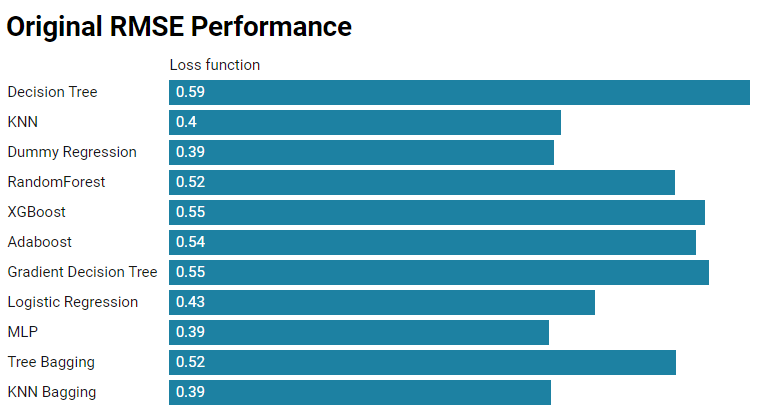
\includegraphics[width=1\linewidth]{original.png}


\section{Hyperparameter selection and model performance}
\textcolor{cyan}{Instruction: \\
In this section, you should describe the way you choose the hyperparameters of your model, also compare the performance of the model with your chosen hyperparamters with models with sub-optimal hyperparameters}\\\\
\textbf{Your work below:}\\
First, we try to normalize the data to see whether a performance improvement could be observed.
In particular, we only normalize features with real-valued meanings, namely Problem View, Correct First Attempt, KC Count, Opportunity Avg, 
Personal Rate, Problem Rate, Step Rate, and KC Rate. However, our expected outcome never emerged. Our result is shown as below.\\
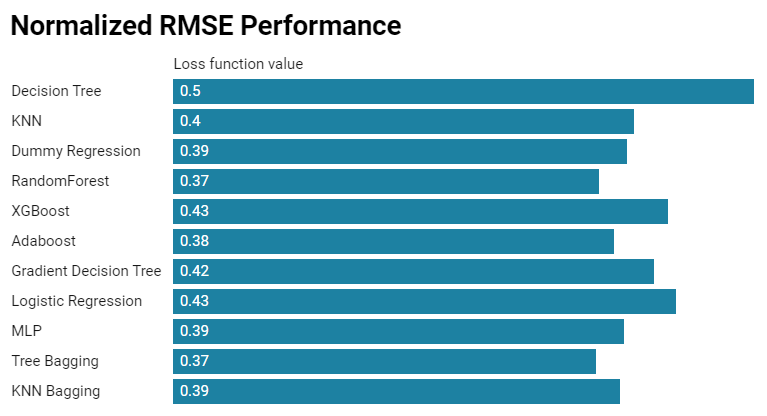
\includegraphics[width=1\linewidth]{normalized.png}

In our next step, we consider optimization of these regressors.
\\
\\In this step,we choose two best performance regressors including RandomForest and Tree bagging to optimize.
\\Initial RandomForest error is 0.51642.After normalization, the optimized RandomForest error is 0.36859.
We optimize RandomForestClassifier's parameters.
\\After calculating and comparing,we find the best parameters for RandomForest.\\
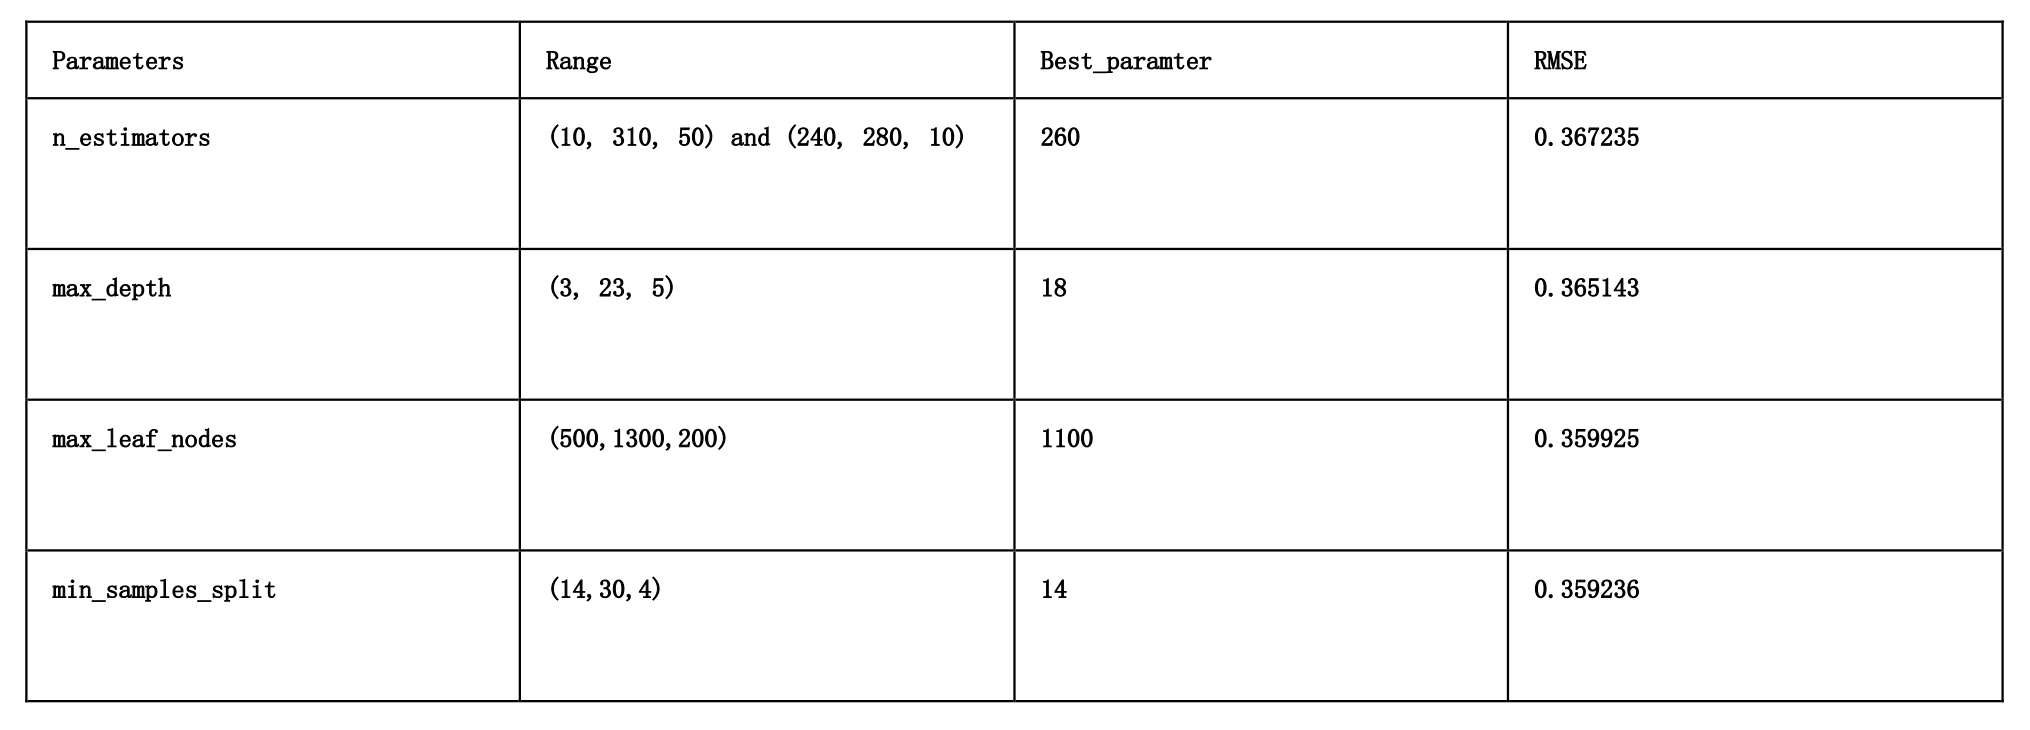
\includegraphics[width=1\linewidth]{optimization.png}
The final optimized RandomForest RMSE is 0.359236.Detailed process and result is in trainlog.md.
\\For Tree bagging,we firstly want to optimize DecisionTree's parameters,but its effect is not as good as we expected.Then we optimize Tree Bagging's parameters.
\\The final optimized Tree Bagging RMSE is 0.363042,which is worse than RandomForest. Detailed process and result is in trainlog.md.
\section{PySpark implementation (optional)}
Our project uses PySpark particularly for Data Cleaning and Feature Engineering. To deal with the large size of training dataset,
we consider using distributed algorithms for our preprocessing in a bid to shorten the running time.\\
Specifically, we make the most of this external library by calling \textbf{pyspark.sql.functions}. We first abstract our algorithm as a function
(particularly when we need to calculate some new features based on data of one certain column), and then call udf to convert our function.
By doing so, we could do our feature engineering with much higher efficiency.\\
We also use \textbf{pyspark.sql.types} to specify our desired data type.
Some aggregation functions are also used in our code.

\end{document}
